\documentclass[11pt]{exam}
\usepackage{listings}
\usepackage[swedish]{babel}
\usepackage[T1]{fontenc} 
\usepackage[utf8]{inputenc} 
\usepackage{algorithm}
\usepackage{algorithmic}


%
%  Created by hwaxxer on 2009-02-23.
%  Copyright (c) 2009 __MyCompanyName__. All rights reserved.
%
%

% This is now the recommended way for checking for PDFLaTeX:
\usepackage{ifpdf}

%\newif\ifpdf
%\ifx\pdfoutput\undefined
%\pdffalse % we are not running PDFLaTeX
%\else
%\pdfoutput=1 % we are running PDFLaTeX
%\pdftrue
%\fi

\ifpdf
\usepackage{subfigure}
\usepackage[pdftex]{graphicx}
\else
\usepackage{graphicx}
\fi

%
%  Update these values for running headers
%
\title{Mästarprov 1 i Algoritmer, Datastrukturer och Komplexitet}
\author{Martin Hwasser}
\runningheader{Martin Hwasser}{}{Mästarprov 1}
\addpoints

\begin{document}
\maketitle
\newpage


% setup standard options for the including code fragments
\lstset{language=Python,numbers=left}

\vspace{0.1in} 

\section{Problem 1: SL-Upplysningen}


\subsection{Problemanalys}
För att lösa problemet kommer vi använda oss av en grafstruktur med hållplatser som hörn, och deras tid i minuter från \textit{t} som kantvikt. Funktionen $time(s,h)$ ger är tidsavståndet från $s$ till $h$, och $min(Q)$ returnerar det hörn i $Q$ som är märkt med den kortaste tiden, och Q implementeras då lämpligen med en prioritetskö. Funktionen $databas(h, t)$ tar en station $h$ och tiden $t$ och returnerar alla platser vi kan åka till ifrån $h$ samt tiden efter $t$ som vi kommer fram. Vi använder oss av Dijkstras algoritm för att hitta den kortaste stigen.
\newline \newline

\subsection{Algoritmbeskrivning}
\textbf{Databas:}

Funktion: \textit{database(h,t)}

\textbf{Indata:} 

En hållplats \textit{h}, och en tidpunkt \textit{t}. 

\textbf{Utdata:}

En lista med alla hållplatser vi kan åka till ifrån \textit{h} och tiden efter \textit{t} som vi kommer fram.
\newline
\textbf{SL-Algoritm:}

\textbf{Indata:}

Starthållplats \textit{s}.

Sökt hållplats \textit{d}.

Tiden \textit{t}.

En tom mängd $M$.

En tom prioritetskö $Q$.

\textbf{Utdata:}

Antal minuter efter \textit{t} som man kommer fram till destinationshållplatsen \textit{d}.

\newpage
\begin{algorithm}
	\caption{: SL-algoritmen}
	\label{alg1}
	\begin{algorithmic} [1]
		\STATE $s \leftarrow 0$
		\STATE $M \leftarrow$ \{$s$\}
		\STATE $t \leftarrow$ tiden
		\STATE $Q.add(databas(s, t))$
		\WHILE[Så länge vi inte har hittat $d$]{$d \notin M$} 
			\STATE $h \leftarrow min(Q)$ \COMMENT{Låt h vara minsta elementet i $Q$}
			\STATE $Q.remove(h)$ \COMMENT{Ta bort $h$ från $Q$}
			\STATE $M.add(h)$ \COMMENT{Lägg till $h$ i $M$}
			\FORALL{hållplatser $h \in databas(h,t)$}
				\IF{$h$ redan har blivit märkt}
					\STATE $h \leftarrow \infty$ \COMMENT{Ty, det finns en kortare väg hit}
				\ELSE 
					\STATE $h \leftarrow time(s,h) + 1$ \COMMENT{Vi har gjort transportbyte, märk $h$ med tiden efter $t$ + 1}
					\STATE $Q.add(h)$
				\ENDIF
			\ENDFOR
		\ENDWHILE
		\STATE return $time(s,d) - 1$
	\end{algorithmic}
\end{algorithm}

\subsection{Algoritmanalys}
SL-algoritmen kommer alltid hitta den kortaste vägen från $s$ till $d$, ty varje stig vi väljer är alltid den kortaste från startnoden, och således kommer vi ha valt den kortaste totala stigen när vi hittar $d$. I värsta fall kommer $for$ $all$-loopen köras $n - 1$ gånger, dvs när en nod är granne med alla andra noder. Vi behöver också räkna med sorteringen i vår prioritetskö när vi lägger till element i varje $for$ $all$-loop, något som sker på $log(n)$ operationer. Den yttre $while$-loopen körs i värsta fall $n - 1$ gånger, vilket sker då $d$ är den sista noden vi hittar. Tidskomplexiteten blir sålunda $O(n \cdot n \cdot log(n)) = O(n^2\cdot log(n))$.

\pagebreak
\newpage

\section{Problem 2: Energisnålt garage för tåg}

\subsection{Problemanalys}
Vi börjar med att konstatera att för varje tåg $i$ med tåglängd $t_i$, gäller att $1 \leq t_i \leq n$. Således krävs för varje tåg $i$ att garagesidan $max(t_i) \leq M \leq n$, ty $M$ måste vara minst lika stort som det längsta tåget $(max(t_i))$, och vi får alltid plats med alla tåg så länge $M$ är lika stort som $n$. För att hitta det optimala $M$ kan vi utföra intervallhalvering, och ansätter först $M = ((n - max(t_i)) / 2) + max(t_i)$. 

\subsection{Algoritmanalys}

Intervallhalvering kommer ha tidskomplexiteten $O(log(n))$ eftersom vi hela tiden förkastar hälften av alla möjliga $M$. Nu behöver vi alltså en algoritm som letar reda på vilken perrong tåget $i$ ska köras in på i $O(n\cdot log(n))$ för att uppfylla kravet på den totala tidskomplexiteten $O(n\cdot log^2(n))$. Vi gör detta med en heapliknande trädstruktur. Vår datastruktur kommer bli ett binärt träd med $log(n)$ nivåer, där löven representerar utrymmet som är kvar i de tillgängliga perrongerna i $M$ (överflödiga perronger nollas enligt bild nedan). Noderna i vårt träd är inledningsvis längden på $M$. Således har vi alltså följande träd om t.ex. $n = 6$:
\begin{center}
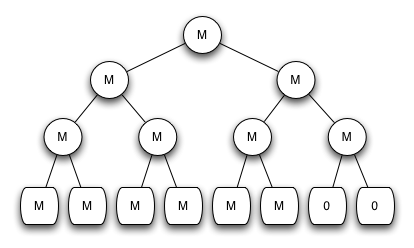
\includegraphics[scale=0.50]{mgraf.png}
\end{center}

Poängen är sedan att parkera tåg $i$ i ett löv så långt till vänster som möjligt där tåget fortfarande får plats, och subtrahera lövets värde med tåglängden $t_i$. Vi vill låta de vänstra noderna vara mindre än de högra, för på så vis förkastar vi vid varje operation hälften av alla perronger. Vi ska placera alla $n$ tåg i trädet, vilket för varje tåg nu går på $log(n)$, och med intervallhalveringen får vi alltså tidskomplexiteten $O(log(n)\cdot n\cdot log(n)) = O(n\cdot log^2(n))$ som vi eftersträvat. 

\subsection{Algoritmbeskrivning}
Vi låter $min \leftarrow max(t_i)$ (längsta tåget) och $max \leftarrow n$ (antalet tåg). Funktionen $generateTree(M)$ genererar ett nytt träd med uppdaterat $M$. Att parkera tågen i trädet görs sedan enligt Algorithm (\ref{alg2}), som anropas med $findMinM(root, t_1, (max - min)/2 + min)$.

\begin{algorithm}
	\caption{: \textbf{findMinM($node, t_i, M$):}}
	\label{alg2}
	\begin{algorithmic} [1]
		\IF[Är tåg $i$ är längre än $M$?]{$node < t_i$}
			\IF[Vi har hittat minsta M]{$(max - M) <= 1$}
				\STATE return max
			\ENDIF
			\STATE $min \leftarrow M$ \COMMENT{Uppdatera $min$}
			
			\STATE $M \leftarrow ((max - min) / 2) + min$. \COMMENT{Öka $M$ med intervallhalvering}
			\STATE $generateTree(M)$ \COMMENT{Generera nytt träd med större M}
			\STATE $findMinM(root, t_1, M)$ \COMMENT{Upprepa processen i nya trädet}
			\STATE break	
		\ELSE
			\IF{$node$ is a leaf}
				\STATE $node \leftarrow node - t_i$ \COMMENT{Dra av tåglängden från perrongen}
				\IF[Har det sista tåget parkerat?]{$i = n$}
					\STATE $max \leftarrow M$ \COMMENT{Uppdatera $max$}
					\STATE $M \leftarrow (max - min) / 2 + min$ \COMMENT{Minska $M$ med intervallhalvering}			
					\STATE $generateTree(M)$ \COMMENT{Generera nytt träd med mindre M}
					\STATE $findMinM(root, t_1, M)$ \COMMENT{Upprepa processen i nya trädet}
					\STATE break
				\ENDIF
				\STATE $findMinM(root,t_{i+1},M)$
			\ELSE
				\IF{$t_i \leq node.left$}
					\STATE $findMinM(node.left, t_i, M)$
					\ELSE
					\STATE $findMinM(node.right, t_i, M)$
					\ENDIF
				\ENDIF
			\STATE $node = max(node.left, node.right)$ \COMMENT{Uppdatera så vi vet hur mycket barnen rymmer}
			\IF[Balansera så att vänstra noden alltid är minst]{$node.left > node.right$}
				\STATE $tmp \leftarrow node.left$
				\STATE $node.left \leftarrow node.right$
				\STATE $node.right \leftarrow tmp$
			\ENDIF
		\ENDIF
	\STATE return $max$ \COMMENT{Vi har hittat rätt eftersom $max$ var senast fungerande $M$}
	\end{algorithmic}
\end{algorithm}


\newpage
	
\section{Problem 3: Hållbart fiske}

\subsection{Problemanalys}
Vi börjar med att konstatera att om $n \leq k$, så använder vi en biljett på varje fiskeplats. Mer intressant är problemet då $n > k$, i vilket fall vi konstruerar en matris $k_{ij}$, där $1 \leq i \leq n$, och $1 \leq j \leq k$, och löser problemet med dynamisk programmering. 

Vi angriper problemet bakifrån, och adderar de olika fiskekvoterna med hjälp av Algorithm (\ref{alg3}). Tanken är att vi summerar fiskekvoter i matrisen utifrån hur vi får stega i den. Hur vi får stega bestäms av att vi åker mellan fiskeplatserna $1$ till $n$ i tur och ordning, och vi skall också använda fiskebiljetterna i tur och ordning samt ej mer än en gång på varje fiskeplats. Dvs, har vi fiskat på $k_{i,j}$, får vi inte fiska vid något fiskeplats $\leq i$ och inte använda en fiskebiljett $\leq j$. Vi måste alltså stega snett nedåt i matrisen varje gång vi använt en fiskebiljett på en fiskeplats. 

\begin{algorithm}
	\caption{: Fiskalgoritmen}
	\label{alg3}
	\begin{algorithmic} [1]
		\FOR{$j = k - 1$ to 1}
			\FOR{$i = n - 1$ to j}
				\IF{$k_{i,j}$ + $k_{i+1,j+1} > k_{i+1,j}$}
					\STATE $k_{i,j} \leftarrow k_{i,j} + k_{i+1,j+1}$
				\ELSE
					\STATE $k_{i,j} \leftarrow k_{i+1,j}$
				\ENDIF
			\ENDFOR
		\ENDFOR
	\end{algorithmic}
\end{algorithm}

\subsection{Algoritmanalys}
Efter detta blir det trivialt att hitta den optimala rutten, eftersom vi summerat fiskekvoterna. Allt vi behöver göra är att leta upp det största värdet i första kolumnen. Om max finns på t.ex. $k_{i,j}$ lägger vi till den fiskeplatsen till en mängd $M$, och letar sedan reda på max i $k_{i+1\rightarrow n,j+1}$ osv, så länge $i + 1 \leq n$ och $j + 1 \leq k$, och lägger till $M$. Tidskomplexiteten blir $O(k\cdot n) + O(k\cdot n) = O(kn)$, ty för varje fiskebiljett $1 \leq j \leq k$ går vi igenom $j \leq i \leq n$ fiskeplatser (det blir en vänstertriangulär matris eftersom vi inte kan använda en biljett $j$ som är större än fiskeplats $i$). Operationerna utförs både vid adderingen samt vid sökandet efter max.

\end{document}

